%!TEX root = ../novoIndex.tex

Considerando a abordagem descrita na solução proposta, os resultados da execução das CNNs aplicadas ao problema de estimação de idade a partir de uma imagem de face são apresentados a seguir.

%
\subsection{Abordagem do TCC1}

A primeira abordagem de treinamento das CNNs constitiu na utilização das imagens da base de dados sem pré-processamento. Conforme mencionado na Seção \ref{subsec:modelos}, os primeiros treinamentos e testes compreenderam as arquiteturas canônicas LeNet e AlexNet com função de ativação \emph{ReLU} na camada de saída, tendo como entrada as imagens do conjunto de dados sem normalização e equalização. Obedecendo ao método de validação cruzada \emph{holdout} previamente mencionado, os resultados da etapa de teste foram obtidos, detalhados na Tabela \ref{tab:results_relu}.

\begin{table}[!ht]
     \caption{Resultados preliminares do treino e teste dos modelos propostos utilizando \emph{ReLU} na camada de saída.}
     \label{tab:results_relu}
     \centering
     \begin{tabular}{l l l}
          \toprule
          Modelo & Épocas &RMSE \\
          \midrule
          LeNet & $95$ & $41.08$ \\
          AlexNet & $55$ & $41.96$\\
          \bottomrule
     \end{tabular}
\end{table}

Ao observar as previsões realizadas para exemplos individuais, percebeu-se uma tendência destas redes após treinamento em preverem valores baixos, indicando possivelmente \emph{underfitting} em virtude do \emph{ReLU dying problem} \cite{djork2015elus, dabal2018elus}. Como alternativa, estes autores sugerem  utilizar variantes da \emph{ReLU} que não exibam saídas nulas, diferentes estratégias de inicialização e regularização de pesos e \emph{batches}, entre outras. Como exposto na Seção \ref{subsec:modelos}, adotou-se a \emph{Leaky ReLU} como função de ativação da camada de saída. Os resultados deste treinamento estão expostos na Tabela \ref{tab:results_leaky}.

\begin{table}[!ht]
     \caption{Resultados preliminares do treino e teste dos modelos propostos utilizando \emph{Leaky ReLU} na camada de saída.}
     \label{tab:results_leaky}
     \centering
     \begin{tabular}{l l l}
          \toprule
          Modelo & Épocas & RMSE \\
          \midrule
          LeNet & $12$ & $41.55$ \\
          AlexNet & $6$ & $14.38$\\
          \bottomrule
     \end{tabular}
\end{table}

Observa-se que houve uma resposta positiva da AlexNet que melhorou a qualidade das previsões para o problema considerado. Porém, observa-se uma tendência desta rede em prever valores médios, o que ainda enseja melhorias. Assim, ainda é necessário investigar outros parâmetros e modelos para o problema em questão.


\subsection{Abordagem 1}%fase2
A primeira abordagem de treinamento das CNNs utilizou as imagens da base de dados com equalização por histograma de frequência, normalizadas, e com $50\%$ de chance de estarem rotacionadas horizontalmente. Conforme mencionado na Seção \ref{subsec:modelos}, os treinamentos e testes compreenderam as arquiteturas canônicas LeNet e AlexNet com funções de ativação \emph{ReLU} e \emph{Leaky ReLU} nas camadas ocultas e de ativação. É importante ressaltar que neste momento não foram utilizadas técnicas de \emph{transfer learning}.

% Explicação da le net, gráficos da le net
A CNN que implementa a arquitetura LeNet com função de ativação \emph{ReLU} foi treinada por 43 épocas, obteve MAE de $14.09$ e RMSE $17.93$. A LeNet com função de ativação \emph{Leaky ReLU} foi treinada por 15 épocas, obteve MAE de $14.44$ anos e RMSE de $18.18$ anos. Os treinamentos duraram aproximadamente $16$ e $12$ horas respectivamente, em uma instância do Google Compute Engine com 4 CPus virtuais e 15 GB de RAM. Os gráficos de treinamento e as retas zero obtidas a partir da apresentação do conjunto de teste aos modelos consolidados podem ser vistos na Figura \ref{fig:lenet-abordagem1}. É possível notar que ambas as redes sofreram com \emph{overfitting} e obtiveram grande margem de erro, no entanto a LeNet que utilizou \emph{Leaky ReLU} como função de ativação obteve um desempenho mais satisfatório.

\begin{figure}[hb!]
	\caption{Resultados do treinamento e teste da CNN LeNet.}\label{fig:lenet-abordagem1}
  \begin{subfigure}[hb]{0.5\linewidth}
    \caption{RMSE de treinamento da arquitetura LeNet utilizando funções de ativação \emph{ReLU}.}
    \label{fig:redeneuralbiologica}
    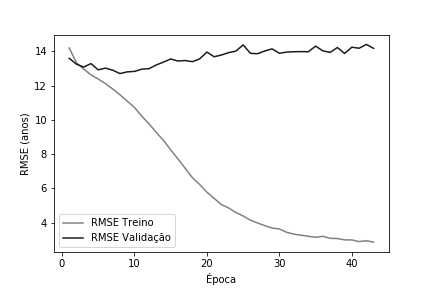
\includegraphics[width=\linewidth]{img/graficos-fase2/fig-history-lenet-relu-data-augmentation-2-1.png}%
  \end{subfigure}%
	\begin{subfigure}[hb]{0.5\linewidth}
		\caption{Reta-0 LeNet \emph{ReLU}.}
		\label{fig:redeneuralbiologica}
		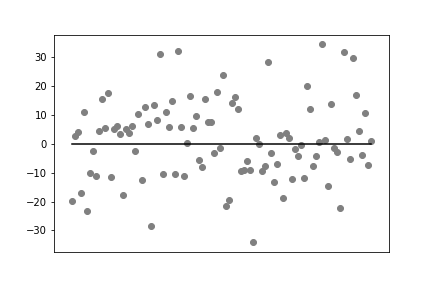
\includegraphics[width=\linewidth]{img/graficos-fase2/fig-reta-0-lenetregressor-relu-data-augmentation-2-1.png}%
	\end{subfigure}\\
  \begin{subfigure}[hb]{0.5\linewidth}
    \caption{RMSE de treinamento da arquitetura LeNet utilizando funções de ativação \emph{Leaky ReLU}.}
    \label{fig:redeneuralbiologica}
    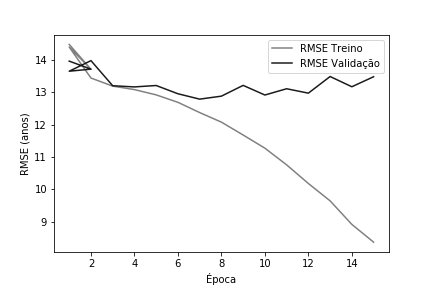
\includegraphics[width=\linewidth]{img/graficos-fase2/fig-history-lenet-lrelu-data-augmentation-2-2.png}
  \end{subfigure}
	\begin{subfigure}[hb]{0.5\linewidth}
		\caption{Reta-0 LeNet \emph{Leaky ReLU}.}
		\label{fig:redeneuralbiologica}
	 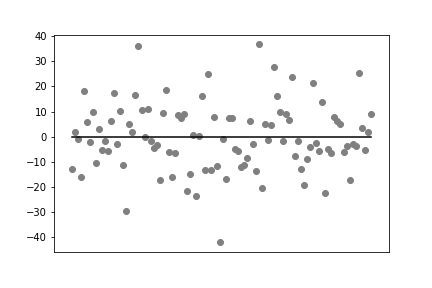
\includegraphics[width=\linewidth]{img/graficos-fase2/fig-reta-0-lenetregressor-lrelu-data-augmentation-2-2.png}
	\end{subfigure}%
\end{figure}

A CNN que implementa a arquitetura AlexNet com função de ativação \emph{ReLU} foi treinada por 10 épocas, obteve MAE de $38.63$ anos e RMSE de $41.22$ anos. A AlexNet com função de ativação \emph{Leaky ReLU} foi treinada por 30 épocas, obteve MAE de $14.44$ anos e RMSE de $15.33$ anos. Os treinamentos duraram aproximadamente $15$ e $38$ horas respectivamente, na mesma instância do Google Compute Engine utilizada para o treinamento das redes LeNet. Os gráficos de treinamento e as retas zero obtidas a partir da apresentação do conjunto de teste aos modelos consolidados podem ser vistos na Figura \ref{fig:alexnet-abordagem1}. É possível notar que a AlexNet que utiliza \emph{ReLU} sofreu de \emph{dying ReLU problem}, o que culminou em previsões iguais a zero para todos os exemplos do conjunto de teste, o que pode ser evidenciado pela ausência total de acertos conforme mostra a Figura \ref{fig:reta0reludying}. Para contornar este problema, a AlexNet que utilizou \emph{Leaky ReLU} como função de ativação foi capaz de convergir para uma solução mais adequada, prevendo idades mais próximas às reais.

\begin{figure}[hb!]
	\caption{Resultados do treinamento e teste da CNN AlexNet.}\label{fig:alexnet-abordagem1}
	\begin{subfigure}[hb]{0.5\linewidth}
		\caption{Treinamento AlexNet \emph{ReLU}.}
		\label{fig:redeneuralbiologica}
		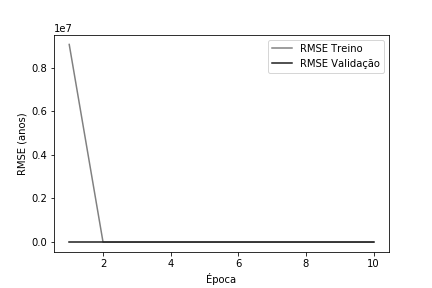
\includegraphics[width=\linewidth]{img/graficos-fase2/fig-history-alexnet-relu-data-augmentation-2-1.png}
	\end{subfigure}
  \begin{subfigure}[hb]{0.5\linewidth}
    \caption{Reta-0 AlexNet \emph{ReLU}.}
    \label{fig:reta0reludying}
    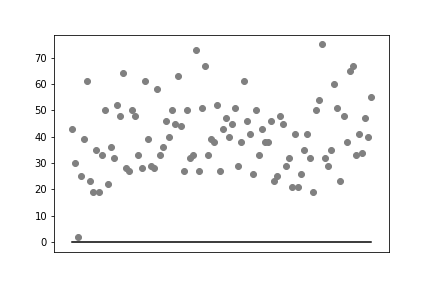
\includegraphics[width=\linewidth]{img/graficos-fase2/fig-reta-0-alexnet-relu-data-augmentation-2-1.png}%
  \end{subfigure}\\
	\begin{subfigure}[hb]{0.5\linewidth}
		\caption{Treinamento AlexNet \emph{Leaky ReLU}.}
		\label{fig:histalexlrelunorm}
    \centering
		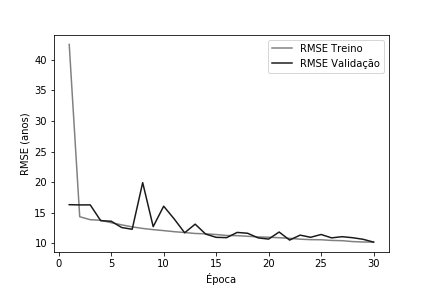
\includegraphics[width=\linewidth]{img/graficos-fase2/fig-history-alexnet-lrelu-data-augmentation-2-2.png}
	\end{subfigure}
  \begin{subfigure}[hb]{0.5\linewidth}
    \caption{Reta-0 AlexNet \emph{Leaky ReLU}.}
    \label{fig:redeneuralbiologica}
    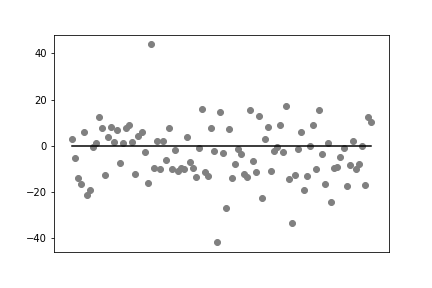
\includegraphics[width=\linewidth]{img/graficos-fase2/fig-reta-0-alexnet-lrelu-data-augmentation-2-2.png}
  \end{subfigure}%
\end{figure}


\begin{figure}[hb!]
	\caption{Redes neurais biológicas.}
	\begin{subfigure}[hb]{0.5\linewidth}
		\caption{Reta-0 Alexnet LRelU com imagens normalizadas e equalizadas}
		\label{fig:histalexlrelunorm}
		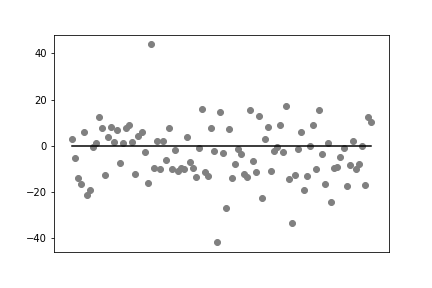
\includegraphics[width=\linewidth]{img/graficos-fase2/fig-reta-0-alexnet-lrelu-data-augmentation-2-2.png}
	\end{subfigure}%
	\begin{subfigure}[hb]{0.5\linewidth}
		\caption{Reta-0 Alexnet ReLU com imagens normalizadas e equalizadas}
		\label{fig:redeneuralbiologica}
		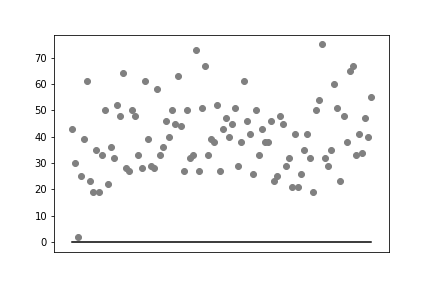
\includegraphics[width=\linewidth]{img/graficos-fase2/fig-reta-0-alexnet-relu-data-augmentation-2-1.png}
	\end{subfigure}
\end{figure}

Obedecendo ao método de validação cruzada \emph{holdout} previamente mencionado, os resultados desta abordagem encontram-se sintetizados na Tabela \ref{tab:results-2}.

\begin{table}[!ht]
	\caption{Resultados do treino e teste dos modelos propostos na Abordagem 1.}
	\label{tab:results-2}
	\begin{adjustbox}{width=1\textwidth}
		\begin{tabular}{l l l l l l l}
			\toprule
			Rede & Função de ativação & Parâmetros & Épocas & Tempo de treinamento & MAE Teste & RMSE Teste \\
			\midrule
			LeNet & \emph{Leaky ReLU} & params & 15 & 12 h & 14.44 & 18.18 \\
			LeNet & \emph{ReLU} & params & 43 & 16 h & 14.09 & 17.93 \\
			AlexNet & \emph{ReLU} & $58.286.145$ & 10 & 15 h & 38.63 & 41.22 \\
			AlexNet & \emph{Leaky ReLU} & params & 30 & 40 h & 15.33 & 18.58 \\
			\bottomrule
		\end{tabular}
	\end{adjustbox}
\end{table}

\subsection{Abordagem 2}

- Mesmas redes
- Normalização das imagens, equalização por histograma -> o que é
- data augmentation ->  mais técnicas de data augmentation

\subsection{Abordagem 3}

Outras arquiteturas
VGG
com transfer learning
1. Retirar última camada (softmax) e adicionar leaky relu
2. Retirar duas últimas camadas (dense e softmax) e adicionar leaky relu
